%%%%%%%%%%%%%%%%%%%%%%%%%%%%%%%%%%%%%%%%%
% baposter Landscape Poster
% LaTeX Template
% Version 1.0 (11/06/13)
%
% baposter Class Created by:
% Brian Amberg (baposter@brian-amberg.de)
%
% This template has been downloaded from:
% http://www.LaTeXTemplates.com
%
% License:
% CC BY-NC-SA 3.0 (http://creativecommons.org/licenses/by-nc-sa/3.0/)
%
%%%%%%%%%%%%%%%%%%%%%%%%%%%%%%%%%%%%%%%%%

%----------------------------------------------------------------------------------------
%	PACKAGES AND OTHER DOCUMENT CONFIGURATIONS
%----------------------------------------------------------------------------------------

\documentclass[landscape,a0paper,fontscale=0.285]{baposter} % Adjust the font scale/size here

\usepackage[numbers]{natbib}

\usepackage{framed} %for easy box around text

\usepackage{graphicx} % Required for including images
\graphicspath{{figures/}} % Directory in which figures are stored

\usepackage{amsmath} % For typesetting math
\usepackage{amssymb} % Adds new symbols to be used in math mode
\usepackage{mathabx}

\usepackage{booktabs} % Top and bottom rules for tables
\usepackage{enumitem} % Used to reduce itemize/enumerate spacing
\usepackage{helvet} % Use the Arial font
\renewcommand{\familydefault}{\sfdefault}
\usepackage[font=small,labelfont=bf]{caption} % Required for specifying captions to tables and figures

\usepackage{xcolor} % use Hex color code

\usepackage{multicol} % Required for multiple columns
\setlength{\columnsep}{1em} % Slightly increase the space between columns
\setlength{\columnseprule}{0mm} % No horizontal rule between columns

\setlength{\textfloatsep}{7pt plus 1.0pt minus 1.0pt}
%\setlength{\floatsep}{7pt plus 1.0pt minus 1.0pt} 
%\setlength{\intextsep}{7pt plus 1.0pt minus 1.0pt} 

\usepackage{enumitem} %allows more customization

\usepackage{tikz} % Required for flow chart
\usetikzlibrary{shapes,arrows} % Tikz libraries required for the flow chart in the template

\newcommand{\compresslist}{ % Define a command to reduce spacing within itemize/enumerate environments, this is used right after \begin{itemize} or \begin{enumerate}
\setlength{\itemsep}{0.3pt}
\setlength{\parskip}{0pt}
\setlength{\parsep}{0pt}
}

\definecolor{darkBlue}{RGB}{16, 27, 34} 
\definecolor{midBlue}{RGB}{66, 111, 138} 
\definecolor{lightBlue}{RGB}{153, 187, 207} 

\begin{document}

\begin{poster}
{
columns=3,
headerborder=closed, % Adds a border around the header of content boxes
colspacing=0.5em, % Column spacing
bgColorOne=white, % Background color for the gradient on the left side of the poster
bgColorTwo=white, % Background color for the gradient on the right side of the poster
borderColor=midBlue, % Border color
headerColorOne=darkBlue, % Background color for the header in the content boxes (left side)
headerColorTwo=lightBlue, % Background color for the header in the content boxes (right side)
headerFontColor=white, % Text color for the header text in the content boxes
boxColorOne=white, % Background color of the content boxes
textborder=roundedleft, % Format of the border around content boxes, can be: none, bars, coils, triangles, rectangle, rounded, roundedsmall, roundedright or faded
eyecatcher=true, % Set to false for ignoring the left logo in the title and move the title left
headerheight=0.13\textheight, % Height of the header
headershape=roundedright, % Specify the rounded corner in the content box headers, can be: rectangle, small-rounded, roundedright, roundedleft or rounded
headerfont=\Large\textsc, % Large, bold and sans serif font in the headers of content boxes
%textfont={\setlength{\parindent}{1em}}, % Uncomment for paragraph indentation
linewidth=2pt % Width of the border lines around content boxes
}
%----------------------------------------------------------------------------------------
%	TITLE SECTION  - done
%----------------------------------------------------------------------------------------
%
{
\includegraphics[height=6em]{epi.png}} % Upload logo of your institution
{\huge{Identifying Cellular Heterogeneity from Optical Reconstruction of Chromatin Architecture}} % Poster title
{\small{Noah G. Burget$^{1,3,4}$, Sora Yoon$^{2,3,4}$, Yeqiao Zhou$^{1,3,4}$, Atishay Jay$^{2,3,4}$, Yiting Chen$^{1,3,4}$, Yimin Sheng$^{1,3,4}$, Golnaz Vahedi$^{2,3,4}$, and R. Babak Faryabi$^{1,3,4}$ \newline 1. Department of Pathology and Laboratory Medicine, 2. Department of Genetics, 3. Institute for Immunology and Immune Health, 4. Epigenetics Institute, University of Pennsylvania, Philadelphia, PA, USA. }} % Author names and institution
{\includegraphics[height=6em]{LabLogo.pdf}} % Second university/lab logo on the right

%----------------------------------------------------------------------------------------
%	Summary  - done
%----------------------------------------------------------------------------------------

\begin{posterbox}[name=section01, column=0, row=0, height=0.4375]{Summary}
While sequencing-based chromatin conformation capture (3C) assays measure genome folding at population-level, Optical Reconstruction of Chromatin Architecture (ORCA) allows for examination of folding at individual alleles. ORCA data can be used to study distances between loci on a chromatin fiber as well as interaction frequency at single alleles. We aim to use this method to elucidate heterogeneity of B cell lymphoma cells. To address this question we compared the performance of several unsupervised machine learning algorithms in identifying subpopulations of B cell lymphoma cells with distinct MYC locus folding. Our studies showed that non-negative matrix factorization (NMF) followed by K-Mean clustering outperforms our approaches in detecting cellular heterogeneity from ORCA data. This analysis shows the existence of three distinct populations of B cell lymphomas with different MYC loci folding. Close examination of the largest subpopulation showed that its average MYC locus folding resembles that of 3C experiments. Together, these data suggest that population-based assays fail to capture the heterogeneity of genome folding and NMF can be used to extract this information from ORCA studies. 
\vspace{0.2 cm}
\end{posterbox}

%----------------------------------------------------------------------------------------
%	Background - done
%----------------------------------------------------------------------------------------

\begin{posterbox}[name=section02, column=0, row=1, below=section01, height=0.5625, above=bottom]{Background}
\begin{center}
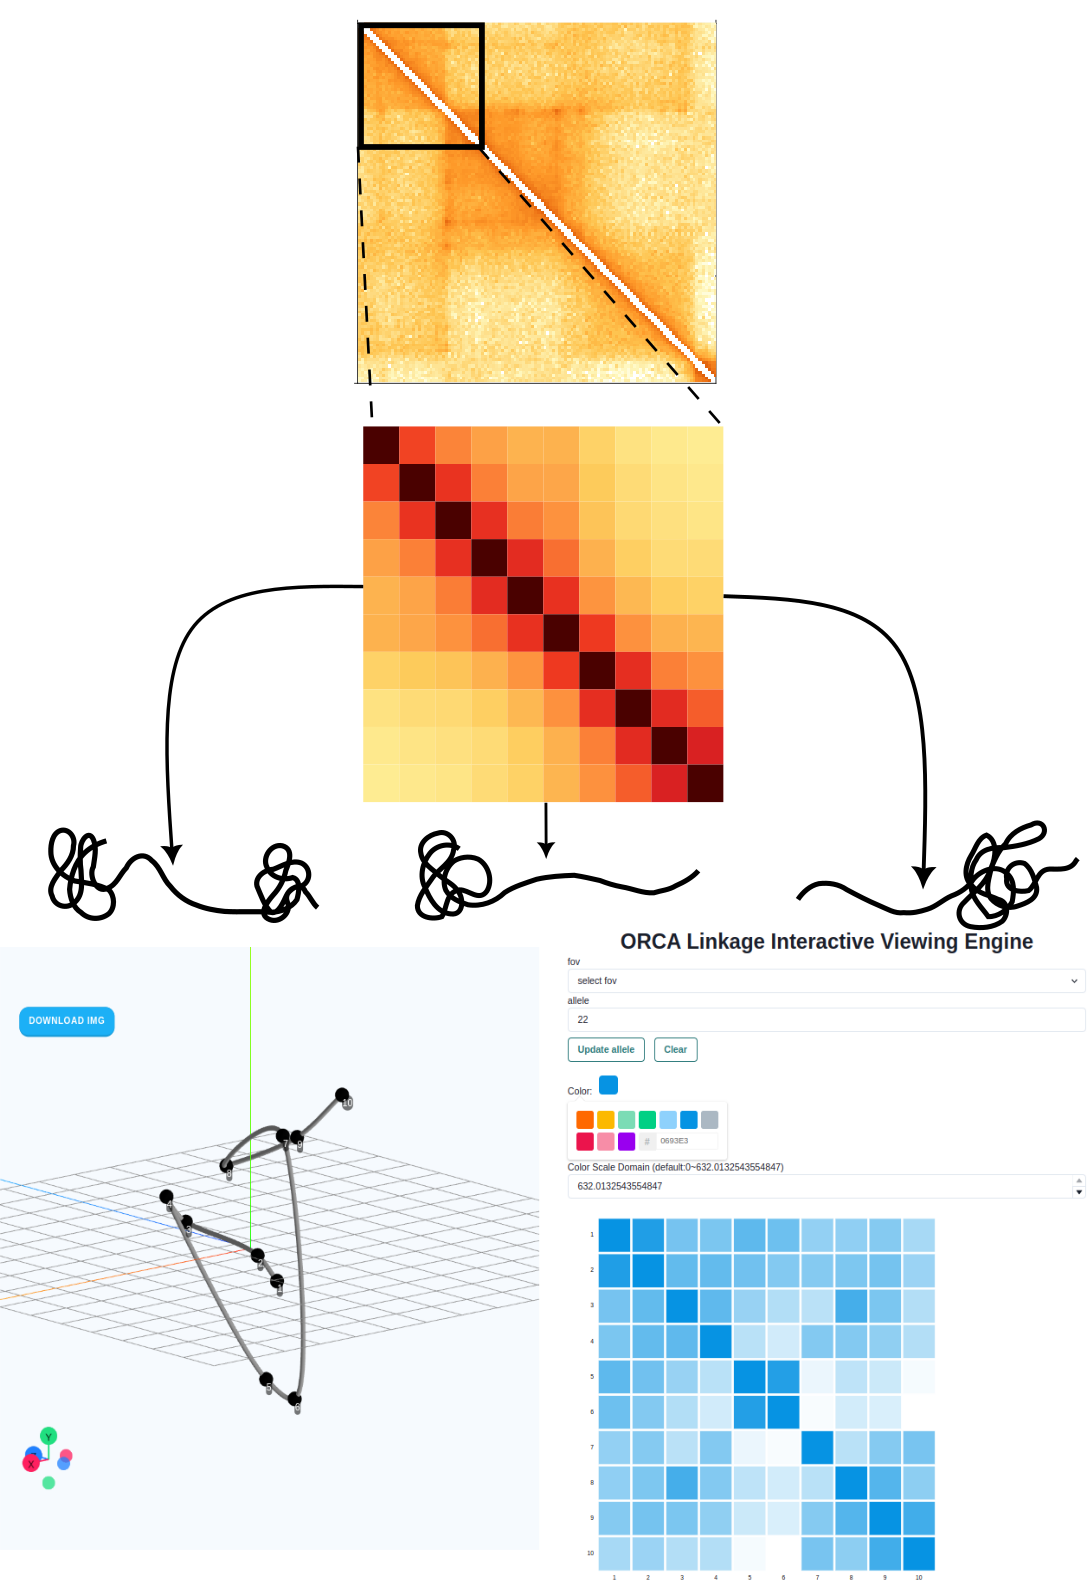
\includegraphics[width=0.8\linewidth, height=290\lineheight]{background.png}
\end{center}
\end{posterbox}

%----------------------------------------------------------------------------------------
%	METHOD 1 (PCA + KMeans)
%----------------------------------------------------------------------------------------

\begin{posterbox}[name=section03, column=1, height=0.333]{Method\ \#1}
\begin{center}
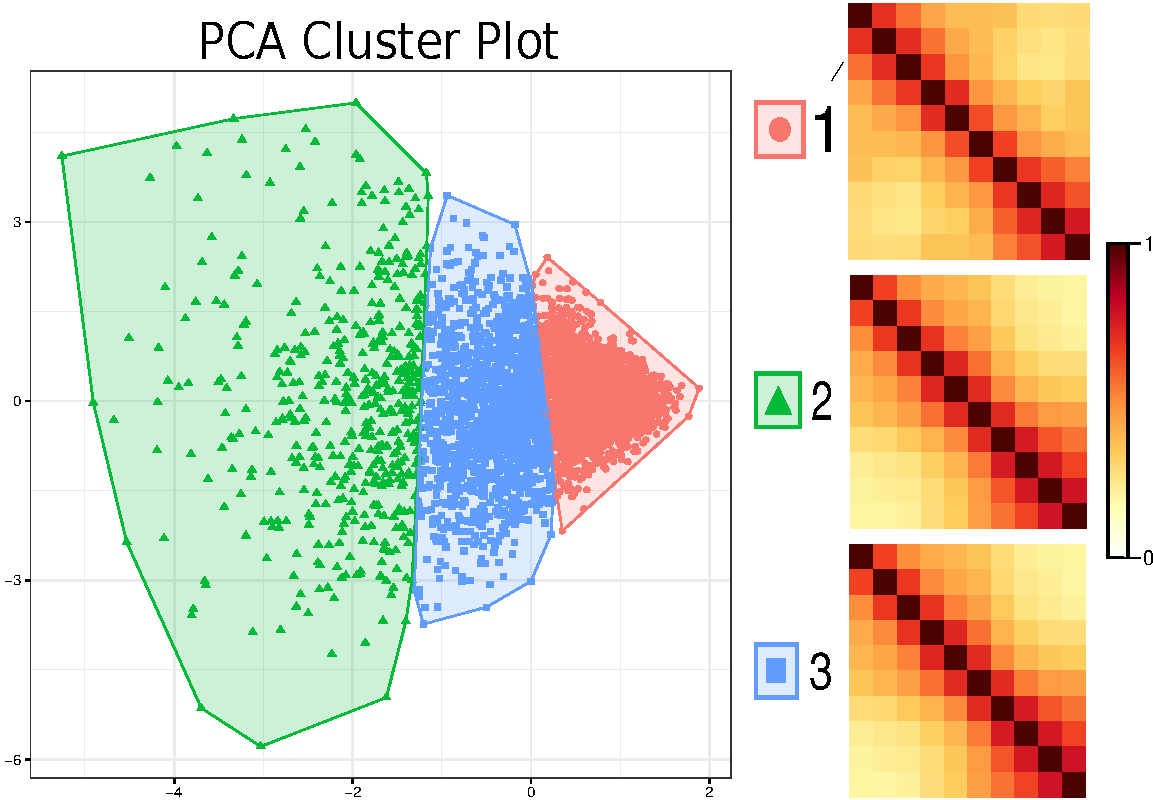
\includegraphics[width=0.9\linewidth, height=160\lineheight]{230902_Granta519cl27_24hdTAG_MYC5p_30mHyb_4phBl_30step_allfits_PCA_clusPlot_matrices.pdf}
\end{center}
\end{posterbox}

%----------------------------------------------------------------------------------------
%	METHOD 2 (UMAP + KMeans)
%----------------------------------------------------------------------------------------

\begin{posterbox}[name=section04, column=1, below=section03, height=0.333]{Method\ \#2}
\begin{center}
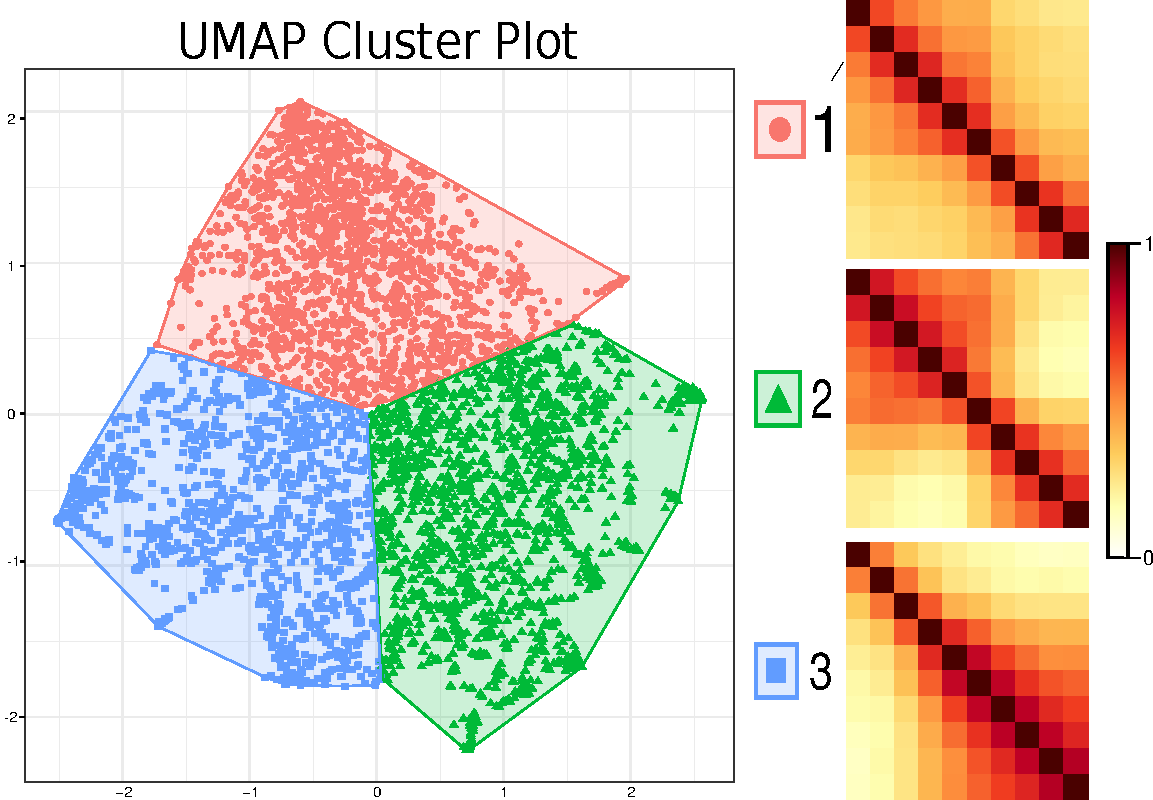
\includegraphics[width=0.9\linewidth, height=160\lineheight]{230902_Granta519cl27_24hdTAG_MYC5p_30mHyb_4phBl_30step_allfits_UMAP_clusPlot_matrices.pdf}
\end{center}
\end{posterbox}
%----------------------------------------------------------------------------------------
%	METHOD 3 (NMF + PAM)
%----------------------------------------------------------------------------------------

\begin{posterbox}[name=section05, column=1, below=section04, height=0.333, above=bottom]{Method\ \#3}
\begin{center}
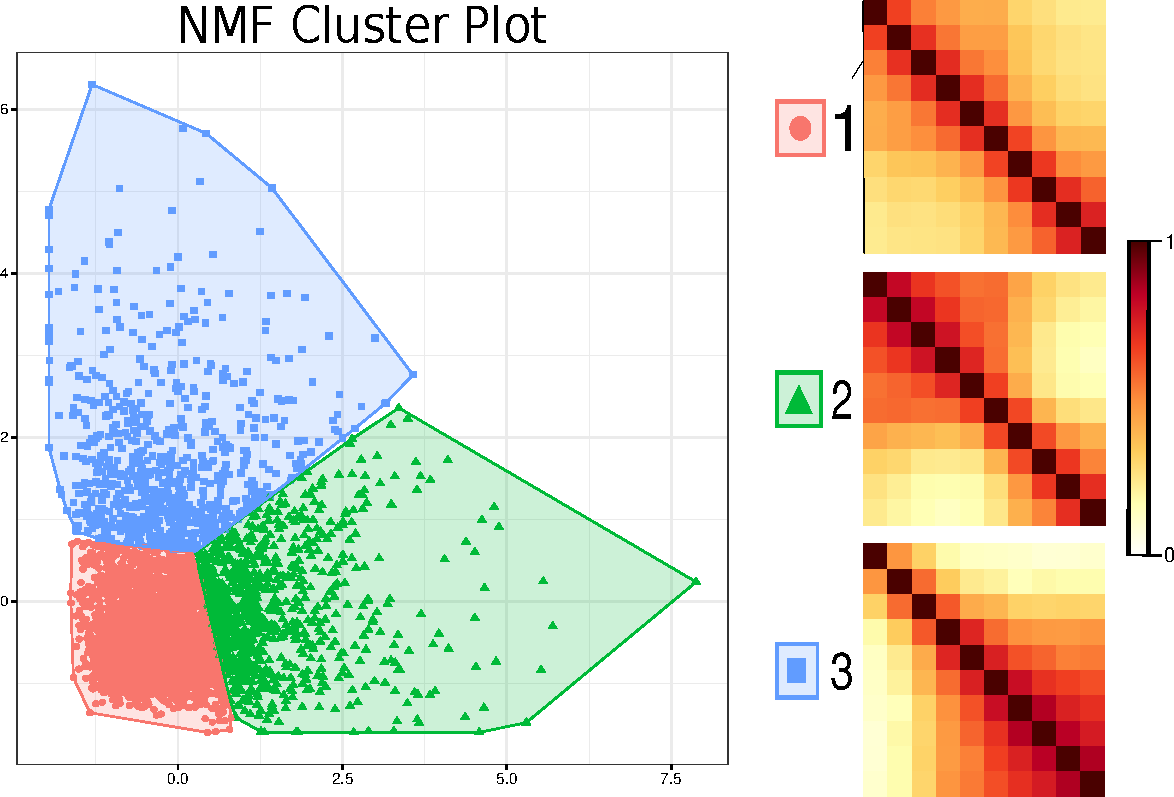
\includegraphics[width=0.9\linewidth, height=155\lineheight]{230902_Granta519cl27_24hdTAG_MYC5p_30mHyb_4phBl_30step_allfits_NMF_clusPlot_matrices.pdf}
\end{center}
\end{posterbox}

%----------------------------------------------------------------------------------------
%	Best method + views
%----------------------------------------------------------------------------------------

\begin{posterbox}[name=section06, column=2, height=0.5]{NMF reveals distinct MYC locus folding}
\begin{center}
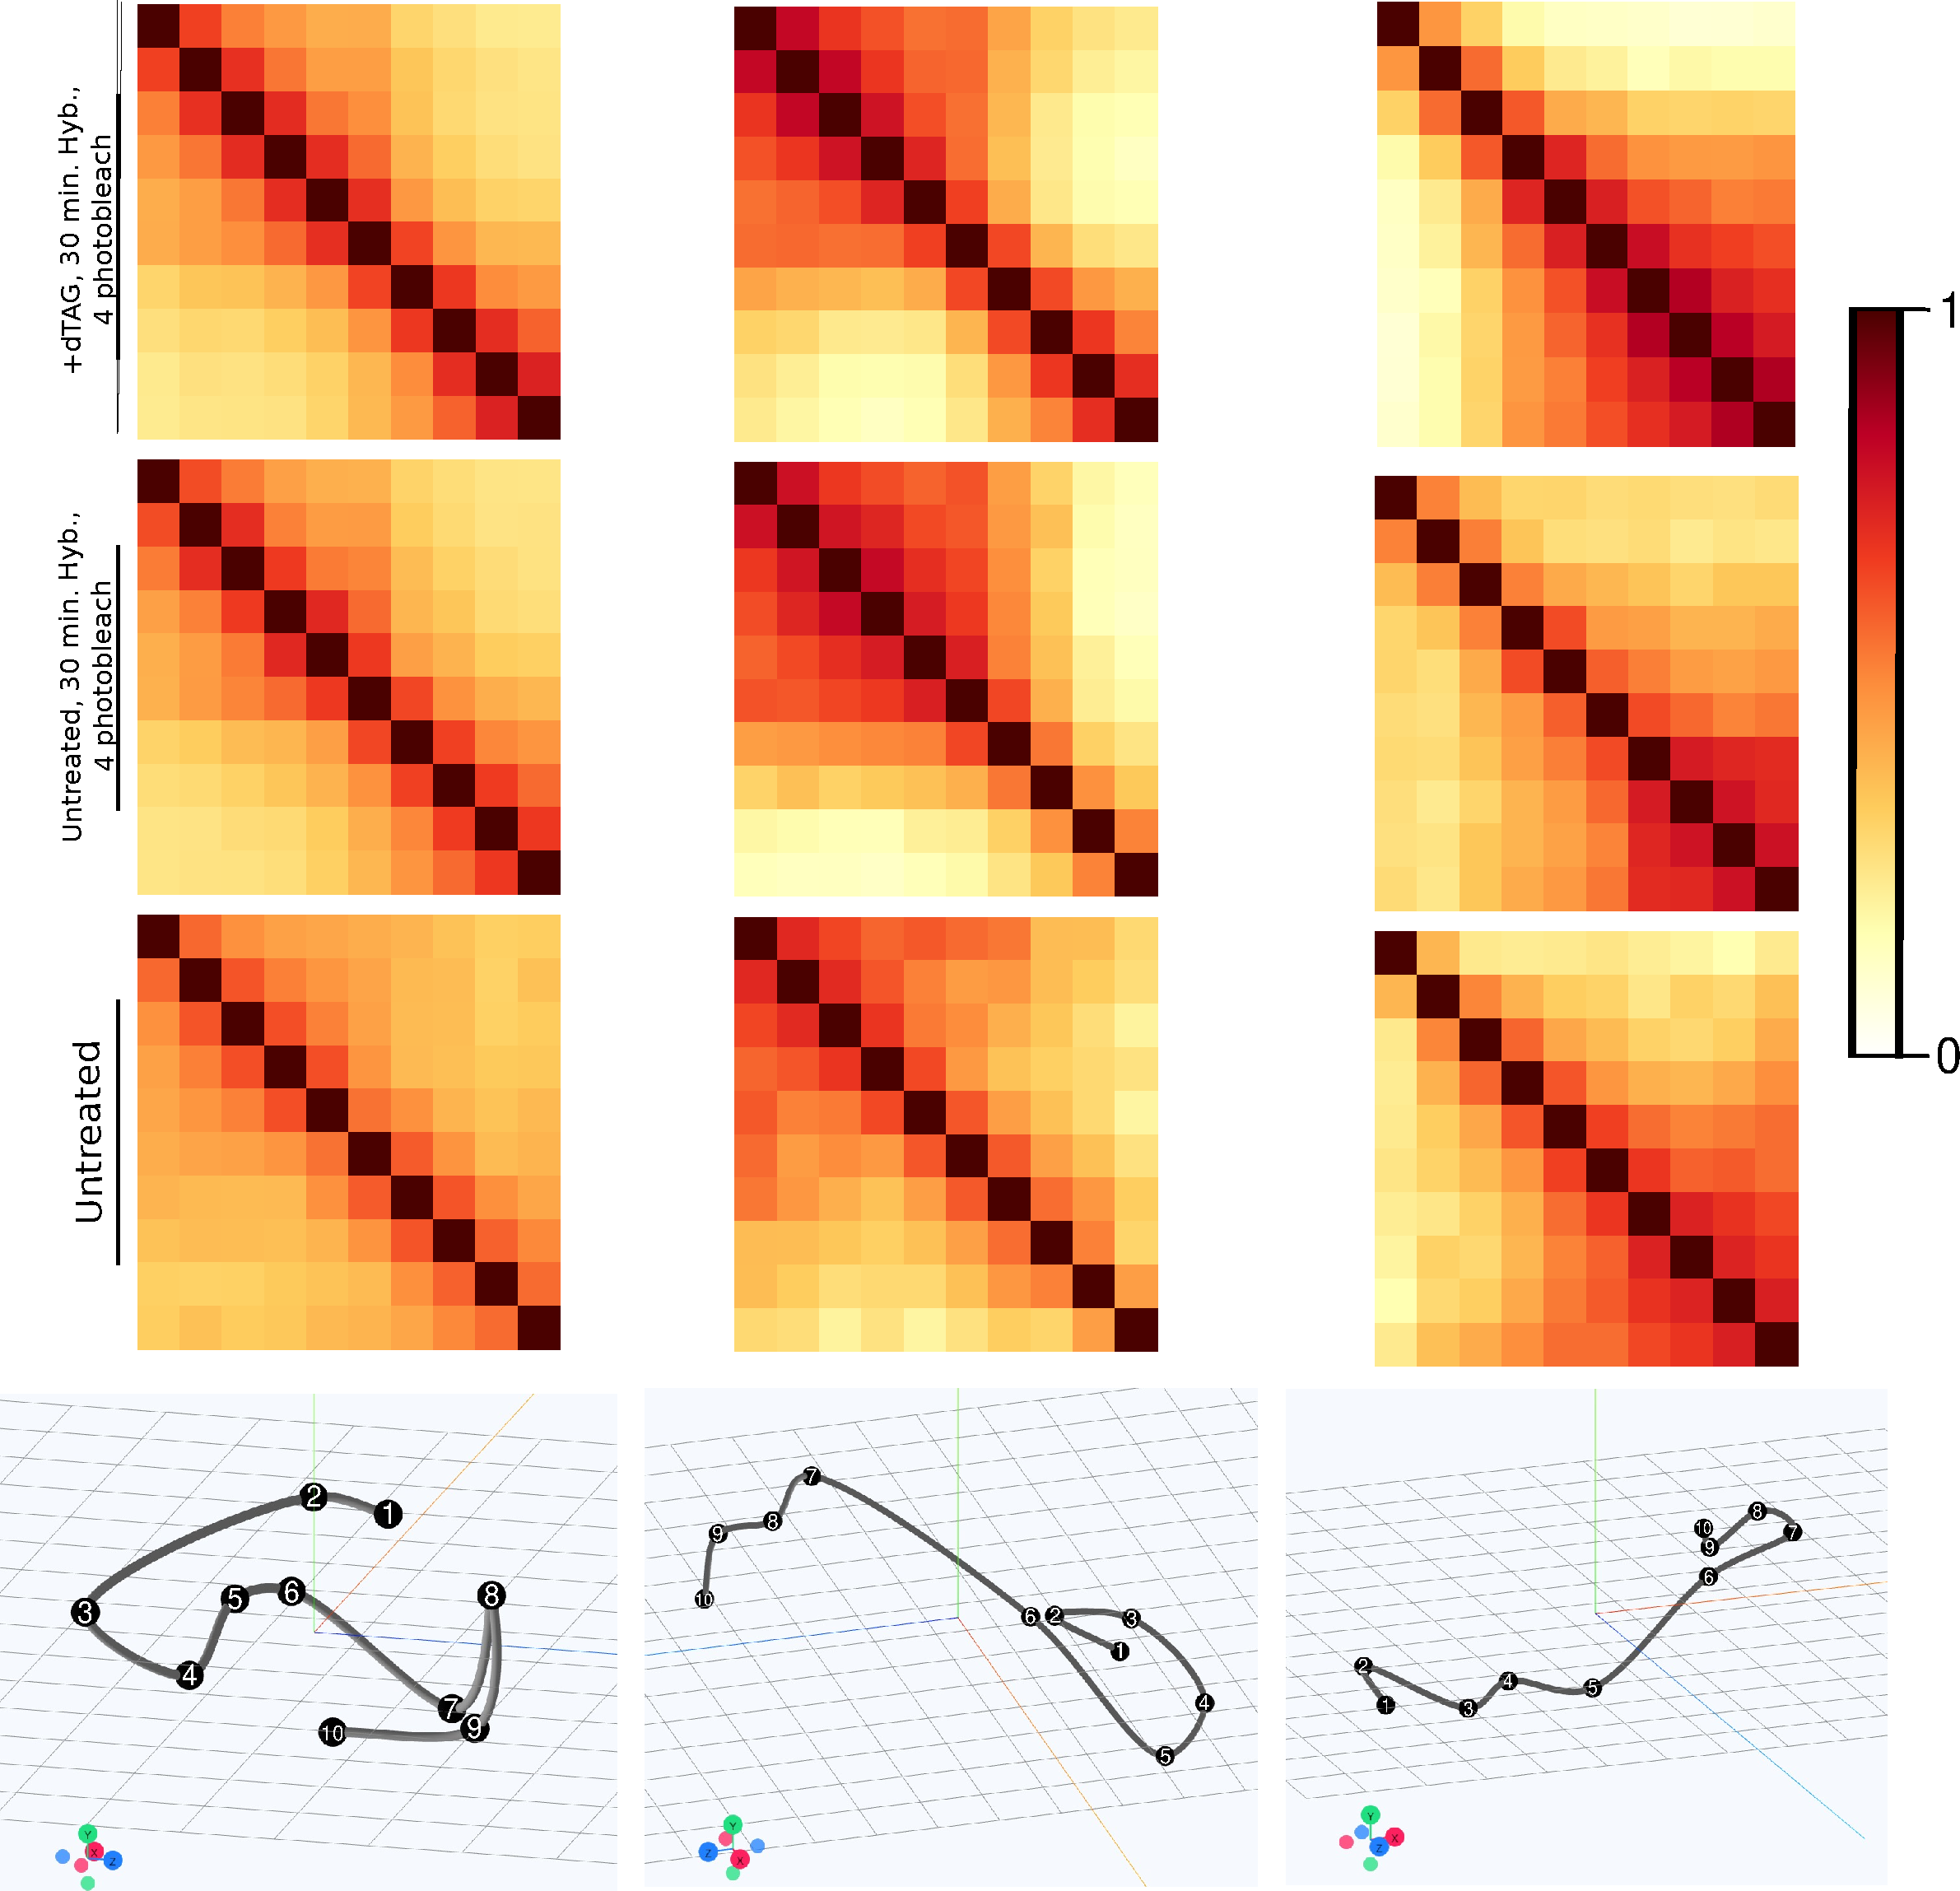
\includegraphics[width=1\linewidth, height=250\lineheight]{bestMethod_nmf_withViews.pdf}
\end{center}
\end{posterbox}

%----------------------------------------------------------------------------------------
%	By Experiment 
%----------------------------------------------------------------------------------------

\begin{posterbox}[name=section07, column=2, below=section06, height=0.5, above=bottom]{Heterogeneity independent of condition}
\begin{center}
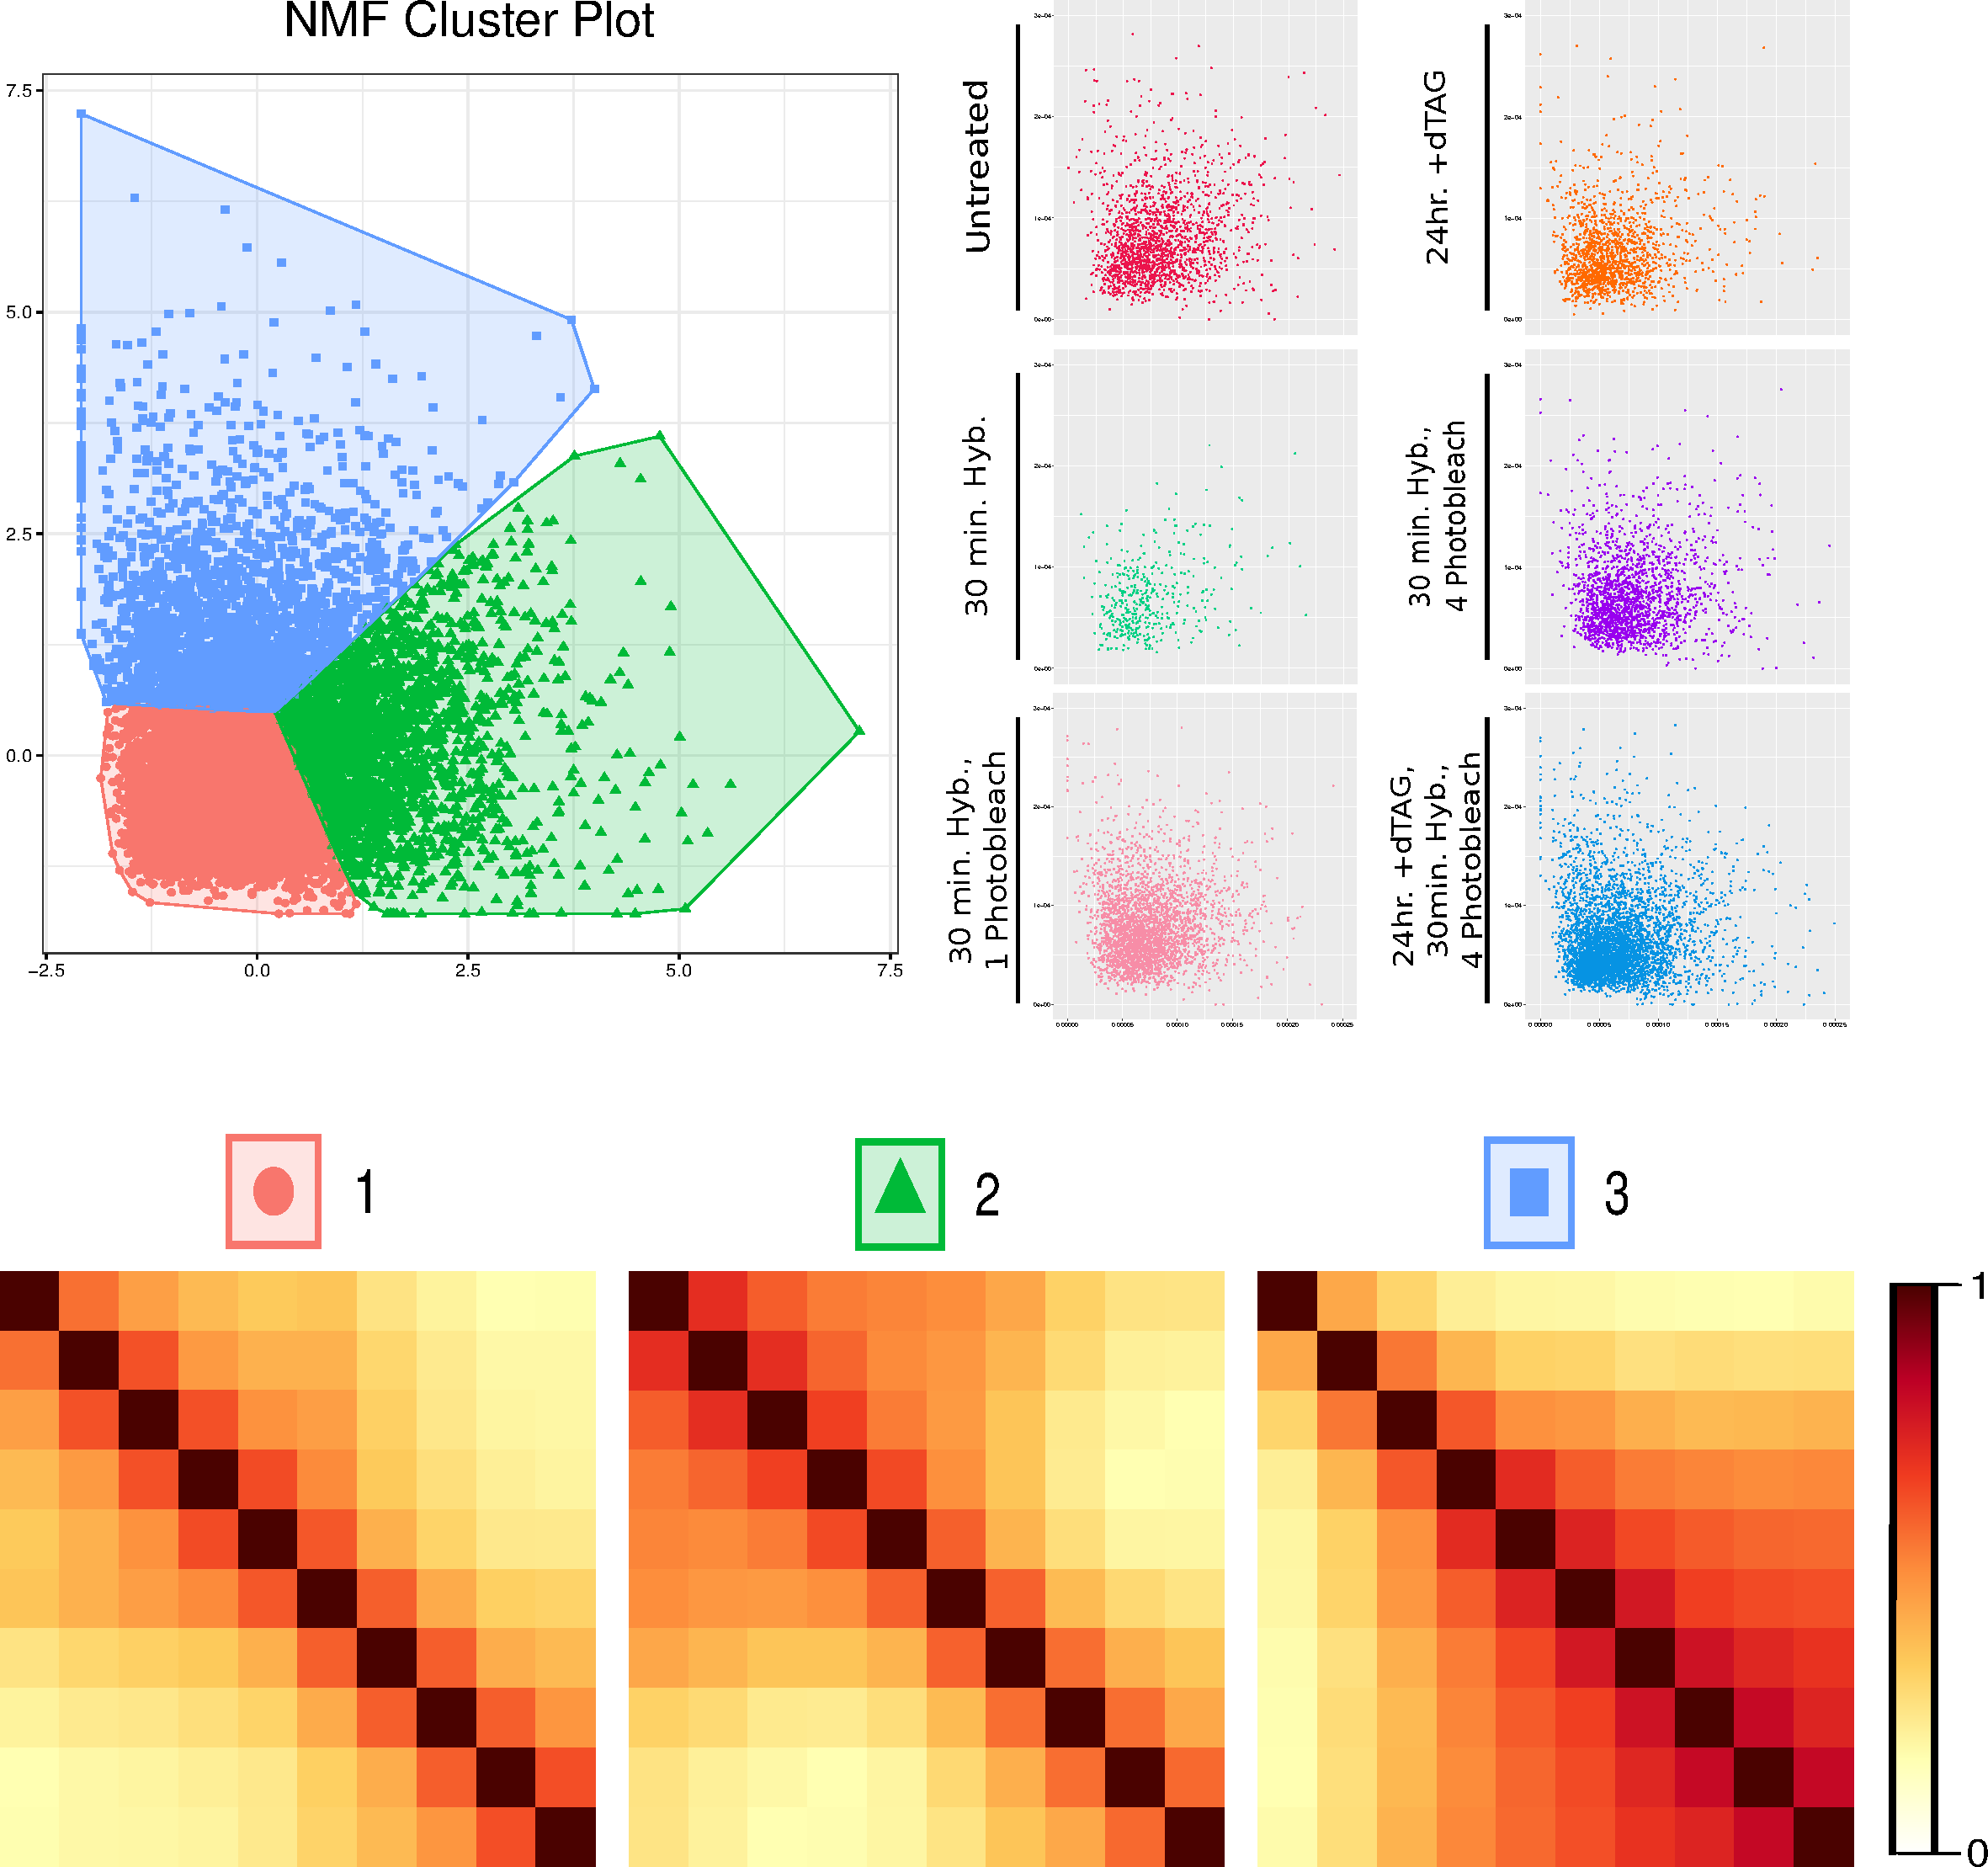
\includegraphics[width=0.9\linewidth, height=250\lineheight]{allSamples_bySample_clusPlot_NMF_matrices.pdf}
\end{center}
\end{posterbox}

%----------------------------------------------------------------------------------------

\end{poster}

\end{document}
